%%%%%%%%%%%%%%%%%%%%%%%%%%%%%%%%%%%%%%%%%
% Beamer Presentation
% LaTeX Template
% Version 1.0 (10/11/12)
%
% This template has been downloaded from:
% http://www.LaTeXTemplates.com
%
% License:
% CC BY-NC-SA 3.0 (http://creativecommons.org/licenses/by-nc-sa/3.0/)
%
%%%%%%%%%%%%%%%%%%%%%%%%%%%%%%%%%%%%%%%%%

%----------------------------------------------------------------------------------------
%    PACKAGES AND THEMES
%----------------------------------------------------------------------------------------

%%TO COMPILE AND GENERATE THE INDEX
%pdflatex TRUST_tutorial.tex
%pdflatex TRUST_tutorial.tex

\documentclass[10pt, hyperref={unicode=true,pdfusetitle, bookmarks=true,bookmarksnumbered=false,bookmarksopen=false, breaklinks=false,pdfborder={0 0 1},backref=true,colorlinks=true,linkcolor=darkblue,pageanchor, urlcolor=darkblue}]{beamer}

\mode<presentation> {

% The Beamer class comes with a number of default slide themes
% which change the colors and layouts of slides. Below this is a list
% of all the themes, uncomment each in turn to see what they look like.

%\usetheme{default}
%\usetheme{AnnArbor}
%\usetheme{Antibes}
%\usetheme{Bergen}
%\usetheme{Berkeley}
%\usetheme{Berlin}
%\usetheme{Boadilla}
\usetheme{CambridgeUS}
%\usetheme{Copenhagen}
%\usetheme{Darmstadt}
%\usetheme{Dresden}
%\usetheme{Frankfurt}
%\usetheme{Goettingen}
%\usetheme{Hannover}
%\usetheme{Ilmenau}
%\usetheme{JuanLesPins}
%\usetheme{Luebeck}
%\usetheme{Madrid}
%\usetheme{Malmoe}
%\usetheme{Marburg}
%\usetheme{Montpellier}
%\usetheme{PaloAlto}
%\usetheme{Pittsburgh}
%\usetheme{Rochester}
%\usetheme{Singapore}
%\usetheme{Szeged}
%\usetheme{Warsaw}

% As well as themes, the Beamer class has a number of color themes
% for any slide theme. Uncomment each of these in turn to see how it
% changes the colors of your current slide theme.

%\usecolortheme{albatross} % bleubleu
%\usecolortheme{beaver} % rouge
%\usecolortheme{beetle} % bleu/gris
%\usecolortheme{crane}  % jaune
%\usecolortheme{dolphin} % bleu
%\usecolortheme{dove}  % blanc
%\usecolortheme{fly} % gris
%\usecolortheme{lily} % bleu
%\usecolortheme{orchid} % bleu
%\usecolortheme{rose} % bleu
%\usecolortheme{seagull} % gris
%\usecolortheme{seahorse} % bleu pale
%\usecolortheme{whale} % bleu
%\usecolortheme{wolverine} % jaune/bleu

%\setbeamertemplate{footline} % To remove the footer line in all slides uncomment this line
%\setbeamertemplate{footline}[page number] % To replace the footer line in all slides with a simple slide count uncomment this line

%\setbeamertemplate{navigation symbols}{} % To remove the navigation symbols from the bottom of all slides uncomment this line

}

\usepackage{graphicx} % Allows including images
\definecolor{darkblue}{HTML}{3535B4}
\definecolor{Greeen}{HTML}{439236}
\definecolor{vert}{HTML}{0ab351}
\definecolor{LightSkyBlue}{HTML}{87CFFA}
\usepackage[T1]{fontenc}
\usepackage{alltt}
\usepackage{tikz}

%----------------------------------------------------------------------------------------
%    TITLE PAGE
%----------------------------------------------------------------------------------------
%\title[Short title]{Long title}
\title[TRUST ICoCo Tutorial V1.7.6]{TRUST ICoCo Tutorial V1.7.6}
% The short title appears at the bottom of every slide, the full title is only on the title page

%\author{John Smith} % Your name
\institute[CEA/DEN/DANS/DM2S/STMF] % Your institution as it will appear on the bottom of every slide, may be shorthand to save space
{
CEA Saclay \\ % Your institution for the title page
\medskip
\textit{Support team: triou@cea.fr} % Your email address
\medskip
}
\date{\today} % Date, can be changed to a custom date


\begin{document}

%%%%%%%%%%%%%%%%%%%%%%%%%%%%%%%%%%%%%%%%%%%%%%%%%%%%%%%%%%%%%%%%%%%%%%%%
\begin{frame}
\titlepage % Print the title page as the first slide
\end{frame}
%%%%%%%%%%%%%%%%%%%%%%%%%%%%%%%%%%%%%%%%%%%%%%%%%%%%%%%%%%%%%%%%%%%%%%%%

%----------------------------------------------------------------------------------------
%    PRESENTATION SLIDES
%----------------------------------------------------------------------------------------
%%%%%%%%%%%%%%%%%%%%%%%%%%%%%%%%%%%%%%%%%%%%%%%%%%%%%%%%%%%%%%%%%%%%%%%%
\begin{frame}
\tableofcontents [hideallsubsections]
%\begin{columns}[c] 
%\column{.45\textwidth}
%\tableofcontents[sections={1-3},hideallsubsections]
%\column{.5\textwidth} 
%\tableofcontents[sections={4-8},hideallsubsections]
%\end{columns}
\end{frame}
%%%%%%%%%%%%%%%%%%%%%%%%%%%%%%%%%%%%%%%%%%%%%%%%%%%%%%%%%%%%%%%%%%%%%%%%



\section{{\bf{Introduction to code coupling and ICoCo}}}
%%%%%%%%%%%%%%%%%%%%%%%%%%%%%%%%%%%%%%%%%%%%%%%%%%%%%%%%%%%%%%%%%%%%%%%%
\begin{frame}
\tableofcontents[currentsection, currentsubsection]
\end{frame}
%%%%%%%%%%%%%%%%%%%%%%%%%%%%%%%%%%%%%%%%%%%%%%%%%%%%%%%%%%%%%%%%%%%%%%%%
%%%%%%%%%%%%%%%%%%%%%%%%%%%%%%%%%%%%%%%%%%%%%%%%%%%%%%%%%%%%%%%%%%%%%%%%
\begin{frame}
\frametitle{Why code coupling?}
\begin{block}{Code coupling ... what for ?}

\begin{columns}[c] 
\column{.6\textwidth}
\begin{itemize}
\item Traditionnaly \textit{numerical simulation codes} focus on a single physics
    \begin{itemize}
    \item [$\circ$] One code for thermics
    \item [$\circ$] Another code for mechanics,
    \item [$\circ$] Etc...
    \end{itemize}
\item Real life studies require the simulation of different physics
    \begin{itemize}
    \item [$\circ$] E.g. nuclear reactor simulations require a blend of: thermics, neutronics, mechanics...
    \end{itemize}
\item Solution? Code coupling!
    \begin{itemize}
    \item [$\circ$] Have different codes communicating one with another...
    \item [$\circ$] And having each of them dealing with its own area of expertise
    \end{itemize}
\end{itemize}

\column{.4\textwidth} 
\begin{figure}[H]
\begin{centering}
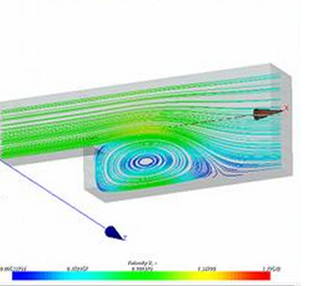
\includegraphics[scale=0.5]{PICTURES/Image1.png}
\par\end{centering}
\end{figure}
\end{columns}

\end{block}
\end{frame}
%%%%%%%%%%%%%%%%%%%%%%%%%%%%%%%%%%%%%%%%%%%%%%%%%%%%%%%%%%%%%%%%%%%%%%%%
%%%%%%%%%%%%%%%%%%%%%%%%%%%%%%%%%%%%%%%%%%%%%%%%%%%%%%%%%%%%%%%%%%%%%%%%
\begin{frame}
\frametitle{Code coupling}
\begin{block}{First approach}

\begin{itemize}
\item An entity driving the complete computation is needed: the \textbf{\textcolor{LightSkyBlue}{supervisor}}
    \begin{itemize}
    \item [$\circ$] Initializes code A and code B
    \item [$\circ$] Loop through code A and code B
    \item [$\circ$] Centralize the exchanges and conversions between A and B
    \item [$\circ$] Supervisor is often usually written from scratch as a C++ file, or a Python script
    \end{itemize}
\item In a dummy approach : supervisor needs to know \textit{both} A and B API
    \begin{itemize}
    \item [$\circ$] Becomes cumbersome if more than 2 codes to couple ...
    \item [$\circ$] Or if one supervisor is meant to run with different pairs of codes (code C, D, E ...)
    \end{itemize}
\end{itemize}

\begin{figure}[h!]
\begin{center}
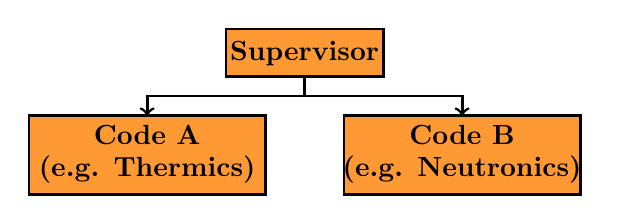
\begin{tikzpicture}[scale=1, line width=1pt]
% box Supervisor
\coordinate (A) at (2.5,1.5) ;
\coordinate (B) at (4.5,1.5) ;
\coordinate (C) at (4.5,2.1) ;
\coordinate (D) at (2.5,2.1) ;
\draw[black,fill=orange!80] (A) -- (B) -- (C) -- (D) -- cycle ;
\draw (3.5,1.5) node[above]{\textbf{Supervisor}} ;
%% box Code A
\begin{scope}
\coordinate (A1) at (0,0) ;
\coordinate (B1) at (3,0) ;
\coordinate (C1) at (3,1) ;
\coordinate (D1) at (0,1) ;
\draw[black,fill=orange!80] (A1) -- (B1) -- (C1) -- (D1) -- cycle ;
\draw (1.5,0.5) node[above]{\textbf{Code A}} ;
\draw (1.5,0.) node[above]{\textbf{(e.g. Thermics)}} ;
\end{scope}
%% box Code B
\begin{scope}
\coordinate (A2) at (4,0) ;
\coordinate (B2) at (7,0) ;
\coordinate (C2) at (7,1) ;
\coordinate (D2) at (4,1) ;
\draw[black,fill=orange!80] (A2) -- (B2) -- (C2) -- (D2) -- cycle ;
\draw (5.5,0.5) node[above]{\textbf{Code B}} ;
\draw (5.5,0.) node[above]{\textbf{(e.g. Neutronics)}} ;
\end{scope}
\draw [->] (3.5,1.5) -- (3.5,1.25) -- (1.5,1.25) -- (1.5,1);
\draw [->] (3.5,1.5) -- (3.5,1.25) -- (5.5,1.25) -- (5.5,1);
\end{tikzpicture}
\end{center}
\end{figure}

\end{block}
\end{frame}
%%%%%%%%%%%%%%%%%%%%%%%%%%%%%%%%%%%%%%%%%%%%%%%%%%%%%%%%%%%%%%%%%%%%%%%%
%%%%%%%%%%%%%%%%%%%%%%%%%%%%%%%%%%%%%%%%%%%%%%%%%%%%%%%%%%%%%%%%%%%%%%%%
\begin{frame}
\frametitle{Code coupling}
\begin{block}{Better: common interface}

\begin{itemize}
\item \underline{\textbf{Idea}}: define a unique \textit{interface} to which each code must comply
    \begin{itemize}
    \item [$\circ$] Only an \textit{interface}, i.e. a contract (=an API) that each code fulfills
    \item [$\circ$] \textit{Implementation} (=plugging the wires) of this interface is tightly linked to the details of the code...
    \end{itemize}
\item Advantages:
    \begin{itemize}
    \item [$\circ$] All codes implementing the (unique) interface can be passed to the supervisor (almost) without modifying it! \textbf{\textcolor{LightSkyBlue}{Versatility}}
    \end{itemize}
\item Cons:
    \begin{itemize}
    \item [$\circ$] Need to implement the interface for each code to be coupled
    \end{itemize}
\end{itemize}

\begin{figure}[h!]
\begin{center}
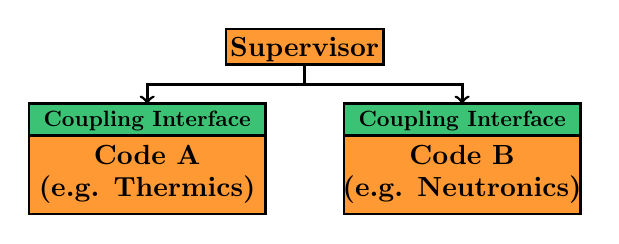
\begin{tikzpicture}[scale=1, line width=1pt]
% box Supervisor
\coordinate (A) at (2.5,1.5) ;
\coordinate (B) at (4.5,1.5) ;
\coordinate (C) at (4.5,1.95) ;
\coordinate (D) at (2.5,1.95) ;
\draw[black,fill=orange!80] (A) -- (B) -- (C) -- (D) -- cycle ;
\draw (3.5,1.4) node[above]{\textbf{Supervisor}} ;
%% box Code A
\begin{scope}
\coordinate (A1) at (0,-0.4) ;
\coordinate (B1) at (3,-0.4) ;
\coordinate (C1) at (3,0.6) ;
\coordinate (D1) at (0,0.6) ;
\coordinate (E1) at (0,1) ;
\coordinate (F1) at (3,1) ;
\draw[black,fill=orange!80] (A1) -- (B1) -- (C1) -- (D1) -- cycle ;
\draw[black,fill=vert!80] (C1) -- (D1) -- (E1) -- (F1)-- cycle ;
\draw (1.5,0.55) node[above,scale=0.8]{\textbf{Coupling Interface}} ;
\draw (1.5,0.1) node[above]{\textbf{Code A}} ;
\draw (1.5,-0.4) node[above]{\textbf{(e.g. Thermics)}} ;
\end{scope}
%% box Code B
\begin{scope}
\coordinate (A2) at (4,-0.4) ;
\coordinate (B2) at (7,-0.4) ;
\coordinate (C2) at (7,0.6) ;
\coordinate (D2) at (4,0.6) ;
\coordinate (E2) at (4,1) ;
\coordinate (F2) at (7,1) ;
\draw[black,fill=orange!80] (A2) -- (B2) -- (C2) -- (D2) -- cycle ;
\draw[black,fill=vert!80] (C2) -- (D2) -- (E2) -- (F2)-- cycle ;
\draw (5.5,0.55) node[above,scale=0.8]{\textbf{Coupling Interface}} ;
\draw (5.5,0.1) node[above]{\textbf{Code B}} ;
\draw (5.5,-0.4) node[above]{\textbf{(e.g. Neutronics)}} ;
\end{scope}
\draw [->] (3.5,1.5) -- (3.5,1.25) -- (1.5,1.25) -- (1.5,1);
\draw [->] (3.5,1.5) -- (3.5,1.25) -- (5.5,1.25) -- (5.5,1);
\end{tikzpicture}
\end{center}
\end{figure}

\end{block}
\end{frame}
%%%%%%%%%%%%%%%%%%%%%%%%%%%%%%%%%%%%%%%%%%%%%%%%%%%%%%%%%%%%%%%%%%%%%%%%
%%%%%%%%%%%%%%%%%%%%%%%%%%%%%%%%%%%%%%%%%%%%%%%%%%%%%%%%%%%%%%%%%%%%%%%%
\begin{frame}
\frametitle{ICoCo}
\begin{block}{Interface for COde COupling}

\begin{itemize}
\item ICoCo is such a coupling interface
\item Stands for Interface for Code Coupling
\item Written in C++
\vspace{0.2cm}
\item Initially designed for simulation codes exhibiting an \textbf{\textcolor{LightSkyBlue}{iterative time loop}} 
\vspace{0.2cm}
\item Presents a set of standard methods whose signature is fixed, with no implementation by default:
    \begin{itemize}
    \item [$\circ$] initializeTimeStep()
    \item [$\circ$] validateTimeStep()
    \item [$\circ$] abortTimeStep()
    \item [$\circ$] ...
    \end{itemize}
\item Uses the notion of field for the exchange of data between codes
    \begin{itemize}
    \item [$\circ$] A field is a set of values supported by a mesh
    \item [$\circ$] A possible implementation: \textbf{MEDCouplingFieldDouble}, from SALOME's MEDCoupling library
    \end{itemize}
\end{itemize}

\end{block}
\end{frame}
%%%%%%%%%%%%%%%%%%%%%%%%%%%%%%%%%%%%%%%%%%%%%%%%%%%%%%%%%%%%%%%%%%%%%%%%
%%%%%%%%%%%%%%%%%%%%%%%%%%%%%%%%%%%%%%%%%%%%%%%%%%%%%%%%%%%%%%%%%%%%%%%%
\begin{frame}
\frametitle{Further reading}
\begin{block}{Meaningful documentation}

\begin{itemize}
\item ICOCO presentation in TRUST documentation:
    \begin{itemize}
    \item [$\circ$] "An Interface for Code Coupling ICoCo v1.2":\\
    \texttt{\$ source /home/triou/env\_TRUST\_X.Y.Z.sh} \\
    \texttt{\$ evince \$TRUST\_ROOT/doc/Kernel/ICoCo\_V1.2.pdf \&}
    \vspace{0.2cm}
    \item [$\circ$] Ask the "APIProblem.pdf" note to triou@cea.fr
    \end{itemize}
\end{itemize}

\end{block}
\end{frame}
%%%%%%%%%%%%%%%%%%%%%%%%%%%%%%%%%%%%%%%%%%%%%%%%%%%%%%%%%%%%%%%%%%%%%%%%



\section{{\bf{TRUST initialization}}}
%%%%%%%%%%%%%%%%%%%%%%%%%%%%%%%%%%%%%%%%%%%%%%%%%%%%%%%%%%%%%%%%%%%%%%%%
\begin{frame}
\tableofcontents[currentsection, currentsubsection]
\end{frame}
%%%%%%%%%%%%%%%%%%%%%%%%%%%%%%%%%%%%%%%%%%%%%%%%%%%%%%%%%%%%%%%%%%%%%%%%
%%%%%%%%%%%%%%%%%%%%%%%%%%%%%%%%%%%%%%%%%%%%%%%%%%%%%%%%%%%%%%%%%%%%%%%%
\begin{frame}
\frametitle{Initialisation of TRUST \& ICoCo environment}
\begin{block}{}

\begin{itemize}
\item Source the TRUST environment:\\
\texttt{\$ source /home/triou/env\_TRUST\_X.Y.Z.sh}
\vspace{0.2cm}

\item To know if the configuration is ok and where are the sources:\\
\texttt{\$ echo \$TRUST\_ROOT}
\vspace{0.2cm}

\item Source the ICoCo environment:\\
\texttt{\$ source \$TRUST\_ROOT/Outils/ICoCo/ICoCo\_src/env\_MEDICoCo.sh}
\vspace{0.2cm}

\item Test if ICoCo is compiled:\\
\texttt{\$ ls \$exec}\\

\item If you obtain "ls: cannot access **/Outils/ICoCo/ICoCo\_src/ICoCo\_opt: No such file or directory", then compile ICoCo\_src:\\
\texttt{\$ cd \$TRUST\_ROOT/Outils/ICoCo/ICoCo\_src}\\
\texttt{\$ baltik\_build\_configure -execute}\\
\texttt{\$ make optim debug }\\
\texttt{\$ source full\_env\_MEDICoCo.sh}
\end{itemize}

\end{block}
\end{frame}
%%%%%%%%%%%%%%%%%%%%%%%%%%%%%%%%%%%%%%%%%%%%%%%%%%%%%%%%%%%%%%%%%%%%%%%%
%%%%%%%%%%%%%%%%%%%%%%%%%%%%%%%%%%%%%%%%%%%%%%%%%%%%%%%%%%%%%%%%%%%%%%%%


\section{{\bf{Basic test case}}}
\subsection{{\bf{ICoCo: without exchange}}}
%%%%%%%%%%%%%%%%%%%%%%%%%%%%%%%%%%%%%%%%%%%%%%%%%%%%%%%%%%%%%%%%%%%%%%%%
\begin{frame}
\tableofcontents[currentsection, currentsubsection]
\end{frame}
%%%%%%%%%%%%%%%%%%%%%%%%%%%%%%%%%%%%%%%%%%%%%%%%%%%%%%%%%%%%%%%%%%%%%%%%
%%%%%%%%%%%%%%%%%%%%%%%%%%%%%%%%%%%%%%%%%%%%%%%%%%%%%%%%%%%%%%%%%%%%%%%%
\begin{frame}
\frametitle{First with TRUST:}
\begin{block}{Launch calculation with TRUST}

\begin{itemize}
\item We create a first reference test case, launched with TRUST.
\item Then we want to launch it with ICoCo and compare the results.
\item Copy the following test case in your repository:\\
\texttt{\$ mkdir ICoCo\_exercises}\\
\texttt{\$ cd ICoCo\_exercises}\\
\texttt{\$ trust -copy Vahl\_Davis\_hexa}
\item Rename the folder to sort your tests:\\
\texttt{\$ mv Vahl\_Davis\_hexa Vahl\_Davis\_hexa\_trust}\\
\texttt{\$ cd Vahl\_Davis\_hexa\_trust}
\item Rename the data file to be consistent with the name of the repository:\\
\texttt{\$ mv Vahl\_Davis\_hexa.data Vahl\_Davis\_hexa\_trust.data}\\
\item Launch calculation:\\
\texttt{\$ trust Vahl\_Davis\_hexa\_trust}\\
\item You obtained a Vahl\_Davis\_hexa\_trust.lml file. We will use it in the following part.
%\item Let do it in parallel also:\\
%\texttt{\$ trust -partition Vahl\_Davis\_hexa}\\
%\texttt{\$ trust PAR\_Vahl\_Davis\_hexa 2}\\
%\item Compare the two results:\\
%\texttt{\$ compare\_lata Vahl\_Davis\_hexa.lml PAR\_Vahl\_Davis\_hexa.lml}\\
%\item The differences are below the threshold: $10^{-5}$!
\end{itemize}

\end{block}
\end{frame}
%%%%%%%%%%%%%%%%%%%%%%%%%%%%%%%%%%%%%%%%%%%%%%%%%%%%%%%%%%%%%%%%%%%%%%%%
%%%%%%%%%%%%%%%%%%%%%%%%%%%%%%%%%%%%%%%%%%%%%%%%%%%%%%%%%%%%%%%%%%%%%%%%
\begin{frame}
\frametitle{With ICoCo}

\begin{block}{Adjusting the data file}
\begin{itemize}
\item Now lets do the same with ICoCo:\\
\texttt{\$ cd ..}\\
\item You are now in your folder "ICoCo\_exercises", create a new directory in order to launch your test case with ICoCo:\\
\texttt{\$ trust -copy Vahl\_Davis\_hexa}\\
\texttt{\$ mv Vahl\_Davis\_hexa Vahl\_Davis\_hexa\_ICoCo}\\
\item Rename the data file to be consistent with the name of the repository:\\
\texttt{\$ cd Vahl\_Davis\_hexa\_ICoCo}\\
\texttt{\$ mv Vahl\_Davis\_hexa.data Vahl\_Davis\_hexa\_ICoCo.data}\\
\item Edit the data file and modify it to add ICoCo instructions:
    \begin{itemize}
    \item [$\circ$] Add the following line after the definition of the dimension:\\
    \textit{Nom ICoCoProblemName Lire ICoCoProblemName pb}
    \item [$\circ$] Comment the "solve pb" line at the end of the data file.
    \end{itemize}
\end{itemize}
\end{block}

\end{frame}
%%%%%%%%%%%%%%%%%%%%%%%%%%%%%%%%%%%%%%%%%%%%%%%%%%%%%%%%%%%%%%%%%%%%%%%%
%%%%%%%%%%%%%%%%%%%%%%%%%%%%%%%%%%%%%%%%%%%%%%%%%%%%%%%%%%%%%%%%%%%%%%%%
\begin{frame}
\frametitle{With ICoCo}

\begin{block}{Creation of the main.cpp file}
\begin{itemize}
%\item Create a parallel data file:\\
%\texttt{\$ trust -partition Vahl\_Davis\_hexa}\\
\item Create the main.cpp which will launch the calculation:\\
\texttt{\$ cp \$TRUST\_ROOT/doc/TRUST/exercices/ICoCo/main1.cpp main.cpp}\\
\item You can edit it and see the main method which creates the objects needed to do the information exchanges.
\item You can use ICoCo with 1 or more processors.
\item Here we use only one processor to solve the problem.
%\item You can also see where the data file and in/output files are set.
%\item Here we only run the calculation with the "while" loop.
\end{itemize}
\end{block}

\begin{block}{Creation of the makefile}
\begin{itemize}
\item Create a makefile for your calculation on 1 proc:\\
\texttt{\$ sh \$project\_directory/share/bin/create\_Makefile 1}
\item Compile it:\\
\texttt{\$ make}
\item It creates an executable "couplage" and a data file "couplage.data".
\end{itemize}

\end{block}
\end{frame}
%%%%%%%%%%%%%%%%%%%%%%%%%%%%%%%%%%%%%%%%%%%%%%%%%%%%%%%%%%%%%%%%%%%%%%%%
%%%%%%%%%%%%%%%%%%%%%%%%%%%%%%%%%%%%%%%%%%%%%%%%%%%%%%%%%%%%%%%%%%%%%%%%
\begin{frame}
\frametitle{With ICoCo}

\begin{block}{Launch calculation}
\begin{itemize}
\item Execute it:\\
\texttt{\$./couplage}
%\texttt{\$ mpirun -np 2 ./couplage}
\item You may obtain the same results as with TRUST executable.
\item Compare it:\\
\texttt{\$ compare\_lata Vahl\_Davis\_hexa\_ICoCo.lml ../Vahl\_Davis\_hexa\_trust/Vahl\_Davis\_hexa\_trust.lml}
%\texttt{\$ compare\_lata PAR\_Vahl\_Davis\_hexa.lml ../Vahl\_Davis\_hexa\_trust/PAR\_Vahl\_Davis\_hexa.lml}
\item The files are the sames!
\end{itemize}

\end{block}
\end{frame}
%%%%%%%%%%%%%%%%%%%%%%%%%%%%%%%%%%%%%%%%%%%%%%%%%%%%%%%%%%%%%%%%%%%%%%%%
%%%%%%%%%%%%%%%%%%%%%%%%%%%%%%%%%%%%%%%%%%%%%%%%%%%%%%%%%%%%%%%%%%%%%%%%



\subsection{{\bf{ICoCo: first input}}}
%%%%%%%%%%%%%%%%%%%%%%%%%%%%%%%%%%%%%%%%%%%%%%%%%%%%%%%%%%%%%%%%%%%%%%%%
\begin{frame}
\tableofcontents[currentsection, currentsubsection]
\end{frame}
%%%%%%%%%%%%%%%%%%%%%%%%%%%%%%%%%%%%%%%%%%%%%%%%%%%%%%%%%%%%%%%%%%%%%%%%
%%%%%%%%%%%%%%%%%%%%%%%%%%%%%%%%%%%%%%%%%%%%%%%%%%%%%%%%%%%%%%%%%%%%%%%%
\begin{frame}
\frametitle{First input with ICoCo}
\begin{block}{Adjusting the main.cpp file}

\begin{itemize}
\item Copy the following test case in your repository:\\
\texttt{\$ cd ICoCo\_exercises}\\
\texttt{\$ cp -r Vahl\_Davis\_hexa\_ICoCo Vahl\_Davis\_hexa\_ICoCo\_exchange}\\
\texttt{\$ cd Vahl\_Davis\_hexa\_ICoCo\_exchange}\\
\item Clean the repository and rename the data file:\\
\texttt{\$ trust -clean}\\
\texttt{\$ mv Vahl\_Davis\_hexa\_ICoCo.data Vahl\_Davis\_hexa\_ICoCo\_exchange.data }\\
%\item We want to create an input of temperature with the first domain. So you have to create a new domain:\\
%\textit{  set<int> dom2\_ids;}
%\item And create objects which will made the input, add the following lines after the "synchronize\_bool(stop,sync\_or);" line:\\
%\textit{  TrioDEC dec\_temperature(dom2\_ids, dom1\_ids);}\\
%\textit{  TrioField Temperature\_field;}
\item We have to add a block in the main.cpp file to made exchanges.
\item Copy the following file in your folder:\\
\texttt{\$ cp \$TRUST\_ROOT/doc/TRUST/exercices/ICoCo/main2.cpp main.cpp}
\end{itemize}

\end{block}
\end{frame}
%%%%%%%%%%%%%%%%%%%%%%%%%%%%%%%%%%%%%%%%%%%%%%%%%%%%%%%%%%%%%%%%%%%%%%%%
%%%%%%%%%%%%%%%%%%%%%%%%%%%%%%%%%%%%%%%%%%%%%%%%%%%%%%%%%%%%%%%%%%%%%%%%
\begin{frame}
\frametitle{First input with ICoCo}
\begin{block}{Adjusting the data file}

\begin{itemize}
\item Then modify the data file Vahl\_Davis\_hexa\_ICoCo\_exchange.data to made the input:
    \begin{itemize}
    \item [$\circ$] Change the line:\\
    "Gauche Paroi\_temperature\_imposee Champ\_Front\_Uniforme 1 10."\\
     to \\
    "Gauche Paroi\_temperature\_imposee ch\_front\_input \{ nb\_comp 1 nom TEMPERATURE\_IN\_DOM probleme pb \}"
    \item [$\circ$] You can see that the name "TEMPERATURE\_IN\_DOM" is the one employed in the main.cpp file.
%    \item [$\circ$] don't forget to update the parallel data file:\\
%    \texttt{\$ trust -partition Vahl\_Davis\_hexa}
    \end{itemize}
\end{itemize}

\end{block}
\end{frame}
%%%%%%%%%%%%%%%%%%%%%%%%%%%%%%%%%%%%%%%%%%%%%%%%%%%%%%%%%%%%%%%%%%%%%%%%
%%%%%%%%%%%%%%%%%%%%%%%%%%%%%%%%%%%%%%%%%%%%%%%%%%%%%%%%%%%%%%%%%%%%%%%%
\begin{frame}
\frametitle{First input with ICoCo}
\begin{block}{Launch calculation}

\begin{itemize}
\item Now we can compile and launch the calculation:\\
\texttt{\$ make}\\
\texttt{\$ ./couplage}
\item You may obtain the same results as with TRUST executable.
\item Compare it:\\
\texttt{\$ compare\_lata Vahl\_Davis\_hexa\_ICoCo\_exchange.lml ../Vahl\_Davis\_hexa\_trust/Vahl\_Davis\_hexa\_trust.lml}
\item The files are the sames! (but not for the first time!!!!!)
\end{itemize}

\end{block}
\end{frame}
%%%%%%%%%%%%%%%%%%%%%%%%%%%%%%%%%%%%%%%%%%%%%%%%%%%%%%%%%%%%%%%%%%%%%%%%
%%%%%%%%%%%%%%%%%%%%%%%%%%%%%%%%%%%%%%%%%%%%%%%%%%%%%%%%%%%%%%%%%%%%%%%%



\subsection{{\bf{ICoCo: on 2 processors}}}
%%%%%%%%%%%%%%%%%%%%%%%%%%%%%%%%%%%%%%%%%%%%%%%%%%%%%%%%%%%%%%%%%%%%%%%%
\begin{frame}
\tableofcontents[currentsection, currentsubsection]
\end{frame}
%%%%%%%%%%%%%%%%%%%%%%%%%%%%%%%%%%%%%%%%%%%%%%%%%%%%%%%%%%%%%%%%%%%%%%%%
%%%%%%%%%%%%%%%%%%%%%%%%%%%%%%%%%%%%%%%%%%%%%%%%%%%%%%%%%%%%%%%%%%%%%%%%
\begin{frame}
\frametitle{First input with ICoCo}
\begin{block}{Adjusting the main.cpp file}

\begin{itemize}
\item Copy the following test case in your repository:\\
\texttt{\$ cd ICoCo\_exercises}\\
\texttt{\$ cp -r Vahl\_Davis\_hexa\_ICoCo\_exchange Vahl\_Davis\_hexa\_ICoCo\_para}\\
\texttt{\$ cd Vahl\_Davis\_hexa\_ICoCo\_para}\\
\item Clean the repository and rename the data file:\\
\texttt{\$ trust -clean}\\
\texttt{\$ rm main.cpp}\\
\texttt{\$ mv Vahl\_Davis\_hexa\_ICoCo\_exchange.data Vahl\_Davis\_hexa\_ICoCo\_para.data }\\
\texttt{\$ trust -partition Vahl\_Davis\_hexa\_ICoCo\_para}\\

\item Copy the following file in your folder:\\
\texttt{\$ cp \$TRUST\_ROOT/doc/TRUST/exercices/ICoCo/main3.cpp main.cpp}\\
\end{itemize}

\end{block}
\end{frame}
%%%%%%%%%%%%%%%%%%%%%%%%%%%%%%%%%%%%%%%%%%%%%%%%%%%%%%%%%%%%%%%%%%%%%%%%
%%%%%%%%%%%%%%%%%%%%%%%%%%%%%%%%%%%%%%%%%%%%%%%%%%%%%%%%%%%%%%%%%%%%%%%%
\begin{frame}
\frametitle{First input with ICoCo}
\begin{block}{Adjusting the main.cpp file}

\begin{itemize}
\item Open the main.cpp file and search for the MPI command lines.
\item Open this file and look where:
    \begin{itemize}
    \item [$\circ$] the processors are added: search for "dom\_ids"
    \item [$\circ$] the names of the data files: search for "data\_file"
    \end{itemize}

\item Compile your new file:\\
\texttt{\$ make}\\
\item To run parallel, you have to use the following mpirun command:\\
\texttt{\$ mpirun -np 2 ./couplage}\\

\item Compare your results with the sequential ones:\\
\texttt{\$ compare\_lata PAR\_Vahl\_Davis\_hexa\_ICoCo\_para.lml ../Vahl\_Davis\_hexa\_trust/Vahl\_Davis\_hexa\_trust.lml}\\
\end{itemize}

\end{block}
\end{frame}
%%%%%%%%%%%%%%%%%%%%%%%%%%%%%%%%%%%%%%%%%%%%%%%%%%%%%%%%%%%%%%%%%%%%%%%%



\section{{\bf{Coupled problem with ICoCo}}}
\subsection{{\bf{ICoCo: without exchange}}}
%%%%%%%%%%%%%%%%%%%%%%%%%%%%%%%%%%%%%%%%%%%%%%%%%%%%%%%%%%%%%%%%%%%%%%%%
\begin{frame}
\tableofcontents[currentsection, currentsubsection]
\end{frame}
%%%%%%%%%%%%%%%%%%%%%%%%%%%%%%%%%%%%%%%%%%%%%%%%%%%%%%%%%%%%%%%%%%%%%%%%
%%%%%%%%%%%%%%%%%%%%%%%%%%%%%%%%%%%%%%%%%%%%%%%%%%%%%%%%%%%%%%%%%%%%%%%%
\begin{frame}
\frametitle{First with TRUST}

\begin{block}{Launch calculation with TRUST}
\begin{itemize}
\item Copy a TRUST test case:\\
\texttt{\$ cd ICoCo\_exercises}\\
\texttt{\$ trust -copy docond\_VEF\_3D}\\
\texttt{\$ mv docond\_VEF\_3D docond\_VEF\_3D\_trust}
\item Launch calculation:\\
\texttt{\$ cd docond\_VEF\_3D\_trust}\\
\texttt{\$ trust docond\_VEF\_3D}
\item Let do it in parallel also:\\
\texttt{\$ trust -partition docond\_VEF\_3D}\\
\texttt{\$ trust PAR\_docond\_VEF\_3D 2}\\
\item Compare the two results:\\
\texttt{\$ compare\_lata docond\_VEF\_3D.lml PAR\_docond\_VEF\_3D.lml}\\
\item The results are the same. Differences are below the threshold: $10^{-5}$!
\end{itemize}
\end{block}

\end{frame}
%%%%%%%%%%%%%%%%%%%%%%%%%%%%%%%%%%%%%%%%%%%%%%%%%%%%%%%%%%%%%%%%%%%%%%%%
%%%%%%%%%%%%%%%%%%%%%%%%%%%%%%%%%%%%%%%%%%%%%%%%%%%%%%%%%%%%%%%%%%%%%%%%
\begin{frame}
\frametitle{Separate a coupled problem into two new problems}
\begin{block}{Separate the meshes}
\begin{itemize}
\item Create your ICoCo test case:\\
\texttt{\$ cd ICoCo\_exercises}\\
\texttt{\$ trust -copy docond\_VEF\_3D}\\
\texttt{\$ mv docond\_VEF\_3D docond\_VEF\_3D\_ICoCo}\\
\texttt{\$ cd docond\_VEF\_3D\_ICoCo}\\
\item Separate mesh and calculation datas in two data files:\\
\texttt{\$ cp docond\_VEF\_3D.data docond\_VEF\_3D\_mesh1.data}\\
\item Edit the file docond\_VEF\_3D\_mesh1.data and remove:
    \begin{itemize}
    \item [$\circ$] the time scheme
    \item [$\circ$] the problem definitions
    \item [$\circ$] the 'scatter' block
    \item [$\circ$] the discretization, medium, gravity definition blocks
    \item [$\circ$] the associations
    \item [$\circ$] the definition and "Read pb1"/"Read pb2" block
    \item [$\circ$] the "fichier pb1"/"fichier pb2" lines
    \item [$\circ$] the "solve" keyword
    \end{itemize}
\end{itemize}
\end{block}
\end{frame}
%%%%%%%%%%%%%%%%%%%%%%%%%%%%%%%%%%%%%%%%%%%%%%%%%%%%%%%%%%%%%%%%%%%%%%%%
%%%%%%%%%%%%%%%%%%%%%%%%%%%%%%%%%%%%%%%%%%%%%%%%%%%%%%%%%%%%%%%%%%%%%%%%
\begin{frame}
\frametitle{Separate a coupled problem into two new problems}
\begin{block}{Separate the meshes}

\begin{itemize}
\item Keep only the domain definitions, meshes and cutting steps.
\item Then create a data file for each domain:\\
\texttt{\$ cp docond\_VEF\_3D\_mesh1.data docond\_VEF\_3D\_mesh2.data }
\item In the file docond\_VEF\_3D\_mesh1.data, keep only the informations of the solide domain.
\item In the file docond\_VEF\_3D\_mesh2.data, keep only the informations of the fluide domain.
\item Uncomment the 'partition' step for each domain.
\item Run these data files:\\
\texttt{\$ trust docond\_VEF\_3D\_mesh1 }\\
\texttt{\$ trust docond\_VEF\_3D\_mesh2 }
\item You must have now the four files:\\
DOM1\_0000.Zones DOM2\_0001.Zones \\
DOM1\_0001.Zones DOM2\_0000.Zones
\end{itemize}

\end{block}
\end{frame}
%%%%%%%%%%%%%%%%%%%%%%%%%%%%%%%%%%%%%%%%%%%%%%%%%%%%%%%%%%%%%%%%%%%%%%%%
%%%%%%%%%%%%%%%%%%%%%%%%%%%%%%%%%%%%%%%%%%%%%%%%%%%%%%%%%%%%%%%%%%%%%%%%
\begin{frame}
\frametitle{Separate a coupled problem into two new problems}

\begin{block}{Run with separated meshes}
\begin{itemize}
\item In docond\_VEF\_3D.data file:
    \begin{itemize}
    \item [$\circ$] remove the mesh and cutting command (which are already in the mesh data file)
    \item [$\circ$] keep the 'scatter' command and uncomment it
    \end{itemize}
\item Launch the calculation:\\
\texttt{\$ trust docond\_VEF\_3D 2}
\item Compare results with previous parallel results:\\
\texttt{\$ compare\_lata docond\_VEF\_3D.lml ../docond\_VEF\_3D\_trust/PAR\_docond\_VEF\_3D.lml }
\item The results are the sames.
\item Separate results in two lml files:
    \begin{itemize}
    \item [$\circ$] add "fichier pb1.lml" in the "Post\_processing" block of the solid domain,
    \item [$\circ$] add "fichier pb2.lml" in the "Post\_processing" block of the fluid domain,
    \end{itemize}
\item Run calculation to create this two files:\\
\texttt{\$ trust docond\_VEF\_3D 2}
\end{itemize}
\end{block}

\end{frame}
%%%%%%%%%%%%%%%%%%%%%%%%%%%%%%%%%%%%%%%%%%%%%%%%%%%%%%%%%%%%%%%%%%%%%%%%
%%%%%%%%%%%%%%%%%%%%%%%%%%%%%%%%%%%%%%%%%%%%%%%%%%%%%%%%%%%%%%%%%%%%%%%%
\begin{frame}
\frametitle{Separate a coupled problem into two new problems}
\begin{block}{Separate data files}

\begin{itemize}
\item Create a data file for the solid domain:\\
\texttt{\$ cp docond\_VEF\_3D.data  docond\_VEF\_3D\_dom1.data }
\item In docond\_VEF\_3D\_dom1.datafile, remove the lines:
    \begin{itemize}
    \item [$\circ$] Probleme\_Couple pbc
    \item [$\circ$] Associate pbc pb1
    \item [$\circ$] Associate pbc pb2
    \end{itemize}
\item Change the following lines:
    \begin{itemize}
    \item [$\circ$] Associate pbc sch $\rightarrow$ Associate pb sch 
    \item [$\circ$] Discretize pbc dis $\rightarrow$ Discretize pb dis
    \item [$\circ$] Solve pbc $\rightarrow$ Solve pb
    \end{itemize}
\item Create a data file for the fluide domain:\\
\texttt{\$ cp docond\_VEF\_3D\_dom1.data docond\_VEF\_3D\_dom2.data}
\item In docond\_VEF\_3D\_dom1.data, keep only the informations about the solid domain (pb1, dom\_solide).
\item Subtitute pb1 $\rightarrow$ pb
\end{itemize}

\end{block}
\end{frame}
%%%%%%%%%%%%%%%%%%%%%%%%%%%%%%%%%%%%%%%%%%%%%%%%%%%%%%%%%%%%%%%%%%%%%%%%
%%%%%%%%%%%%%%%%%%%%%%%%%%%%%%%%%%%%%%%%%%%%%%%%%%%%%%%%%%%%%%%%%%%%%%%%
\begin{frame}
\frametitle{Separate a coupled problem into two new problems}
\begin{block}{Separate data files}

\begin{itemize}
\item In docond\_VEF\_3D\_dom2.data, keep only the informations about the fluide domain (pb2, dom\_fluide).
\item Subtitute pb2 $\rightarrow$ pb
\item You can see that the heat exchange is made on the "Paroi\_echange1" boundary for solid domain and "Paroi\_echange2" boundary for the fluid domain.
\item Modify docond\_VEF\_3D\_dom1.data file to have:\\
\textit{Paroi\_echange1 paroi\_contact pb Paroi\_echange2} \\
$\rightarrow$ \\
\textit{Paroi\_echange1 paroi\_temperature\_imposee Champ\_Front\_Uniforme 1 50.}
\item Modify docond\_VEF\_3D\_dom2.data file to have:\\
\textit{Paroi\_echange2 paroi\_contact pb Paroi\_echange1} \\
$\rightarrow$ \\
\textit{Paroi\_echange2 paroi\_temperature\_imposee Champ\_Front\_Uniforme 1 50.}
\end{itemize}

\end{block}
\end{frame}
%%%%%%%%%%%%%%%%%%%%%%%%%%%%%%%%%%%%%%%%%%%%%%%%%%%%%%%%%%%%%%%%%%%%%%%%
%%%%%%%%%%%%%%%%%%%%%%%%%%%%%%%%%%%%%%%%%%%%%%%%%%%%%%%%%%%%%%%%%%%%%%%%
\begin{frame}
\frametitle{Separate a coupled problem into two new problems}

\begin{block}{Separate data files}
\begin{itemize}
\item Run docond\_VEF\_3D\_dom1.data and docond\_VEF\_3D\_dom2.data in parallel:\\
\texttt{\$ trust docond\_VEF\_3D\_dom1 2 }\\
\texttt{\$ trust docond\_VEF\_3D\_dom2 2 }
\item The two problems must run.
\item Notice that there is no coupling at all for the moment.
\end{itemize}
\end{block}

\begin{block}{Adjusting data files}
\begin{itemize}
\item To create the ICoCo problem, just after 'dimension 3', add in docond\_VEF\_3D\_dom1.data and docond\_VEF\_3D\_dom2.data:\\
'Nom ICoCoProblemName Lire ICoCoProblemName pb'
\item Remove 'Solve pb' because the solving step will be made by ICoCo.
\end{itemize}
\end{block}

\end{frame}
%%%%%%%%%%%%%%%%%%%%%%%%%%%%%%%%%%%%%%%%%%%%%%%%%%%%%%%%%%%%%%%%%%%%%%%%
%%%%%%%%%%%%%%%%%%%%%%%%%%%%%%%%%%%%%%%%%%%%%%%%%%%%%%%%%%%%%%%%%%%%%%%%
\begin{frame}
\frametitle{Run with ICoCo}



\begin{block}{Creation of the main.cpp file}
\begin{itemize}
\item We have to create a new executable which will use our data files.
\item Copy the following main.cpp file in your repository:\\
\texttt{\$ cp \$TRUST\_ROOT/doc/TRUST/exercices/ICoCo/main3.cpp main.cpp }
\item Open this file and look where:
    \begin{itemize}
    \item [$\circ$] the processors are added: search for "dom1\_ids"
    \item [$\circ$] the names of the data files: search for "data\_file"
    \item [$\circ$] the loop to iterate on time steps: search for "while"
    \end{itemize}
\end{itemize}
\end{block}

\end{frame}
%%%%%%%%%%%%%%%%%%%%%%%%%%%%%%%%%%%%%%%%%%%%%%%%%%%%%%%%%%%%%%%%%%%%%%%%
%%%%%%%%%%%%%%%%%%%%%%%%%%%%%%%%%%%%%%%%%%%%%%%%%%%%%%%%%%%%%%%%%%%%%%%%
\begin{frame}
\frametitle{Run with ICoCo}

\begin{block}{Compiling and launching}
\begin{itemize}
\item Create a makefile to compile your main.cpp file:\\
\texttt{\$ sh \$project\_directory/share/bin/create\_Makefile 4}
\item Compile the main.cpp file:\\
\texttt{\$ make}
\item Launch calculation:\\
\texttt{\$ mpirun -np 4 ./couplage}
\item Compare the results to the results of the coupled problem:\\
\texttt{\$ compare\_lata pb1.lml docond\_VEF\_3D\_dom1.lml}\\
\texttt{\$ compare\_lata pb2.lml docond\_VEF\_3D\_dom2.lml}
\item As expected, there are differences between the results because there is no coupling here, we impose the temperature in the data files.
\end{itemize}
\end{block}

\end{frame}
%%%%%%%%%%%%%%%%%%%%%%%%%%%%%%%%%%%%%%%%%%%%%%%%%%%%%%%%%%%%%%%%%%%%%%%%



\subsection{{\bf{ICoCo: one way coupling}}}
%%%%%%%%%%%%%%%%%%%%%%%%%%%%%%%%%%%%%%%%%%%%%%%%%%%%%%%%%%%%%%%%%%%%%%%%
\begin{frame}
\tableofcontents[currentsection, currentsubsection]
\end{frame}
%%%%%%%%%%%%%%%%%%%%%%%%%%%%%%%%%%%%%%%%%%%%%%%%%%%%%%%%%%%%%%%%%%%%%%%%
%%%%%%%%%%%%%%%%%%%%%%%%%%%%%%%%%%%%%%%%%%%%%%%%%%%%%%%%%%%%%%%%%%%%%%%%
\begin{frame}
\frametitle{Run with ICoCo}

\begin{block}{Adjusting data file}
\begin{itemize}
\item Now we want to send the temperature from the Paroi\_echange2 boundary of the domain dom2 to the Paroi\_echange1 boundary of the domain dom1.
\item Create a new directory:\\
\texttt{\$ cd ICoCo\_exercises}\\
\texttt{\$ cp -r docond\_VEF\_3D\_ICoCo docond\_VEF\_3D\_ICoCo\_coupling1}\\
\texttt{\$ cd docond\_VEF\_3D\_ICoCo\_coupling1}\\


\item In the docond\_VEF\_3D\_dom2.data data file, add in the "Definition\_champs" block of the post-processings:\\
\texttt{ \hspace{0.2cm} TEMPERATURE\_OUT\_DOM2 Interpolation \{             } \\
\texttt{ \hspace{0.5cm}    localisation elem                                } \\
\texttt{ \hspace{0.5cm}    domaine dom\_fluide\_boundaries\_Paroi\_echange2 } \\
\texttt{ \hspace{0.5cm}    source refChamp \{ Pb\_Champ pb temperature \}   } \\
\texttt{ \hspace{0.2cm} \}                                                  } \\
where "dom\_fluide\_boundaries\_Paroi\_echange2" is a predefined name for the boundary Paroi\_echange2 of the domain dom2.
\end{itemize}
\end{block}

\end{frame}
%%%%%%%%%%%%%%%%%%%%%%%%%%%%%%%%%%%%%%%%%%%%%%%%%%%%%%%%%%%%%%%%%%%%%%%%
%%%%%%%%%%%%%%%%%%%%%%%%%%%%%%%%%%%%%%%%%%%%%%%%%%%%%%%%%%%%%%%%%%%%%%%%
\begin{frame}
\frametitle{Run with ICoCo}

\begin{block}{Adjusting data file}
\begin{itemize}
\item In the docond\_VEF\_3D\_dom1.data data file, change the boundary condition on the 'Paroi\_echange1' boundary to:\\
Paroi\_echange1 paroi\_temperature\_imposee ch\_front\_input \{ nb\_comp 1 nom TEMPERATURE\_IN\_DOM1 probleme pb \}
\item Copy the main.cpp file for this exchange:\\
\texttt{\$ cp \$TRUST\_ROOT/doc/TRUST/exercices/ICoCo/main4.cpp main.cpp }
\item Compare the new main.cpp file to the previous one:\\
\texttt{\$ tkdiff main.cpp ../docond\_VEF\_3D\_ICoCo/main.cpp }
\item You can see where the new fields TEMPERATURE\_IN\_DOM1 and TEMPERATURE\_OUT\_DOM2 added to the data files, are used in a new part which makes exchanges.
\item Notice that we use two new objects: one TrioDEC object and one TrioField object.
\item Some comments are written to help you.
\end{itemize}
\end{block}

\end{frame}
%%%%%%%%%%%%%%%%%%%%%%%%%%%%%%%%%%%%%%%%%%%%%%%%%%%%%%%%%%%%%%%%%%%%%%%%
%%%%%%%%%%%%%%%%%%%%%%%%%%%%%%%%%%%%%%%%%%%%%%%%%%%%%%%%%%%%%%%%%%%%%%%%
\begin{frame}
\frametitle{Run with ICoCo}

\begin{block}{Adjusting data file}
\begin{itemize}
\item Compile the main.cpp file:\\
\texttt{\$ make}
\item Launch calculation:\\
\texttt{\$ mpirun -np 4 ./couplage}
\item Compare results with those without coupling:\\
\texttt{\$ compare\_lata docond\_VEF\_3D\_dom1.lml ../docond\_VEF\_3D\_ICoCo/docond\_VEF\_3D\_dom1.lml }\\
\texttt{\$ compare\_lata docond\_VEF\_3D\_dom2.lml ../docond\_VEF\_3D\_ICoCo/docond\_VEF\_3D\_dom2.lml }\\
\item The results on the domain dom2 are the same as this calculation made only one more post-traitment.
\item But we can see that the coupling works well because the results on the domain dom1 changes.
\end{itemize}
\end{block}

\end{frame}
%%%%%%%%%%%%%%%%%%%%%%%%%%%%%%%%%%%%%%%%%%%%%%%%%%%%%%%%%%%%%%%%%%%%%%%%



\subsection{{\bf{ICoCo: two way coupling}}}
%%%%%%%%%%%%%%%%%%%%%%%%%%%%%%%%%%%%%%%%%%%%%%%%%%%%%%%%%%%%%%%%%%%%%%%%
\begin{frame}
\tableofcontents[currentsection, currentsubsection]
\end{frame}
%%%%%%%%%%%%%%%%%%%%%%%%%%%%%%%%%%%%%%%%%%%%%%%%%%%%%%%%%%%%%%%%%%%%%%%%
%%%%%%%%%%%%%%%%%%%%%%%%%%%%%%%%%%%%%%%%%%%%%%%%%%%%%%%%%%%%%%%%%%%%%%%%
\begin{frame}
\frametitle{Run with ICoCo}

\begin{block}{Adjusting data file}
\begin{itemize}
\item Two way coupling for thermal problems should use Dirichlet and Neumann boundary conditions (using only Dirichlet boundary conditions for coupling both sides would not work).
\item So we want to send the heat flux from the Paroi\_echange1 boundary of the domain dom1 to the Paroi\_echange2 boundary of the domain dom2.
\item Create a new directory:\\
\texttt{\$ cd ICoCo\_exercises}\\
\texttt{\$ cp -r docond\_VEF\_3D\_ICoCo\_coupling1 docond\_VEF\_3D\_ICoCo\_coupling2}\\
\texttt{\$ cd docond\_VEF\_3D\_ICoCo\_coupling2}\\
\item Inspire you of the previous part to make a Neumann boundary condition (heat flux imposed):

\end{itemize}
\end{block}

\end{frame}
%%%%%%%%%%%%%%%%%%%%%%%%%%%%%%%%%%%%%%%%%%%%%%%%%%%%%%%%%%%%%%%%%%%%%%%%
%%%%%%%%%%%%%%%%%%%%%%%%%%%%%%%%%%%%%%%%%%%%%%%%%%%%%%%%%%%%%%%%%%%%%%%%
\begin{frame}
\frametitle{Run with ICoCo}

\begin{block}{Adjusting data file}
\begin{itemize}
\item In the docond\_VEF\_3D\_dom1.data data file, add in the "Definition\_champs" block of the post-processings:\\
\texttt{ \hspace{0.2cm} FLUX\_SURFACIQUE\_OUT\_DOM1 Interpolation \{             } \\
\texttt{ \hspace{0.5cm}    localisation elem                                     } \\
\texttt{ \hspace{0.5cm}    domaine dom\_fluide\_boundaries\_Paroi\_echange1      } \\
\texttt{ \hspace{0.5cm}    source Morceau\_equation \{                           } \\
\texttt{ \hspace{0.7cm}        type operateur numero 0 option flux\_surfacique\_bords } \\
\texttt{ \hspace{0.7cm}        source refChamp \{ Pb\_Champ pb temperature \} } \\
\texttt{ \hspace{0.5cm}    \}                                                  } \\
\texttt{ \hspace{0.2cm} \}                                                     } \\
where "dom\_solide\_boundaries\_Paroi\_echange1" is a predefined name for the boundary Paroi\_echange1 of the domain dom1.

\item In the docond\_VEF\_3D\_dom2.data data file, change the boundary condition on the 'Paroi\_echange2' boundary to:\\
Paroi\_echange2 paroi\_flux\_impose ch\_front\_input \{ nb\_comp 1 nom FLUX\_SURFACIQUE\_IN\_DOM2 probleme pb \}
\end{itemize}
\end{block}

\end{frame}
%%%%%%%%%%%%%%%%%%%%%%%%%%%%%%%%%%%%%%%%%%%%%%%%%%%%%%%%%%%%%%%%%%%%%%%%
%%%%%%%%%%%%%%%%%%%%%%%%%%%%%%%%%%%%%%%%%%%%%%%%%%%%%%%%%%%%%%%%%%%%%%%%
\begin{frame}
\frametitle{Run with ICoCo}

\begin{block}{Adjusting data file}
\begin{itemize}
\item Modify the main.cpp file to add a new exchange:\\
    \begin{itemize}
    \item [$\circ$] Create a new TrioDEC object to made exchange from domain dom2 to domain dom1: \\
    \textit{TrioDEC dec\_flux\_surfacique2(dom2\_ids, dom1\_ids);}
    \item [$\circ$] Create a new TrioField object: \\
    \textit{TrioField field\_flux\_surfacique2;}
    \item [$\circ$] Add code lines into the while loop to made this exchange of informations.
    \end{itemize}
\item You can have a look at the main5.cpp file for this exchange:\\
\texttt{\$ cp \$TRUST\_ROOT/doc/TRUST/exercices/ICoCo/main5.cpp main5.cpp }

\item Compare it to the previous one:\\
\texttt{\$ tkdiff main5.cpp ../docond\_VEF\_3D\_ICoCo\_coupling1/main.cpp }
\item You can see the use of the new fields FLUX\_SURFACIQUE\_IN\_DOM2 and FLUX\_SURFACIQUE\_OUT\_DOM1 added to the data files.

\end{itemize}
\end{block}

\end{frame}
%%%%%%%%%%%%%%%%%%%%%%%%%%%%%%%%%%%%%%%%%%%%%%%%%%%%%%%%%%%%%%%%%%%%%%%%
%%%%%%%%%%%%%%%%%%%%%%%%%%%%%%%%%%%%%%%%%%%%%%%%%%%%%%%%%%%%%%%%%%%%%%%%
\begin{frame}
\frametitle{Run with ICoCo}

\begin{block}{Adjusting data file}
\begin{itemize}
\item Compile your main.cpp file:\\
\texttt{\$ make}
\item Launch calculation:\\
\texttt{\$ mpirun -np 4 ./couplage}
\item Compare results with the first ones:\\
\texttt{\$ compare\_lata docond\_VEF\_3D\_dom1.lml ../docond\_VEF\_3D\_ICoCo/pb1.lml }\\
\texttt{\$ compare\_lata docond\_VEF\_3D\_dom2.lml ../docond\_VEF\_3D\_ICoCo/docond\_VEF\_3D\_dom2.lml }\\

\end{itemize}
\end{block}

\end{frame}
%%%%%%%%%%%%%%%%%%%%%%%%%%%%%%%%%%%%%%%%%%%%%%%%%%%%%%%%%%%%%%%%%%%%%%%%










%  Post\_processings \{
%    dom2_post {
%      Definition_champs {
%        TEMPERATURE_OUT Interpolation
%        {
%          localisation elem
%          domaine dom_fluide_boundaries_Paroi_echange2
%          source refChamp { Pb_Champ pb temperature }
%        }
%      }
%      format lata  Champs dt_post 0.05
%      {
%        vitesse elem
%        vitesse som
%                                temperature elem
%                                temperature som
%      }
%    }
%    bord_dom2_post {
%       format lata
%       domaine dom_fluide_boundaries_Paroi_echange2
%       Champs dt_post 0.05
%       {
%        temperature elem # aux sommets plante #
%        pression_pa elem
%        vitesse som
%       }
%      }
%  }

%# dans docond_VEF_3D_dom1.data, ajouter :
%  Post_processings
%  {
%    dom1_post # uniquement pour visu #
%    {
%      format lata
%      Champs dt_post 0.05
%      {
%                                temperature elem
%                                temperature som
%      }
%    }
%    bord_dom1_post # uniquement pour visu #
%    {
%       format lata
%       domaine dom_solide_boundaries_Paroi_echange1
%       Champs dt_post 0.05
%       { 
%        temperature elem # aux sommets plante #
%        temperature som
%       }
%     }
%  }


%mpirun -np 4 ./couplage # OK mais toujours pas d'echange fait
%# main.cpp
%# decommenter l169 à 276
%# supprimer tt ce qui concerne la pression
%# trouver la ligne contenant la definition d'un objet du type "TrioDEC"
%TrioDEC dec_vit_in_chaude(dom2_ids, dom1_ids);
%definition le champ TrioDEC dec_vit_in_chaude comme transferant des données du dom2_ids au dom1_ids
%renommer tout les  dec_vit_in_chaude en dec_temperature
%idem pour : TrioField vit_chaude;
%renommer vit_chaude en field_temperature
%VITESSE_OUT -> TEMPERATURE_OUT
%vitesse_in -> TEMPERATURE_IN
%retirer les commandes contenant des save_vit
%vmin -> tmin
%vmax -> tmax
%cerr<<" vitesse min"<<vmin << " max "<<vmax<<endl; -> cerr<<" temperature min"<<tmin << " max "<<tmax<<endl;
%#       Paroi_echange1 paroi_temperature_imposee Champ_Front_Uniforme 1 50. #
%      Paroi_echange1    paroi_temperature_imposee ch_front_input { nb_comp 1 nom TEMPERATURE_IN probleme pb }


%  vector<string> inputnames= T->getInputFieldsNames();
%  for (unsigned int ii=0;ii<inputnames.size();ii++)
%    cout<<data_file<<"  Field Input  " <<inputnames[ii]<<endl;
%  cout<<endl;




%%%%%%%%%%%%%%%%%%%%%%%%%%%%%%%%%%%%%%%%%%%%%%%%%%%%%%%%%%%%%%%%%%%%%%%%
%\begin{frame}
%\begin{columns}[c] 
%\column{.45\textwidth}
%\tableofcontents[sections={1-3},currentsection, currentsubsection]
%\column{.5\textwidth} 
%\tableofcontents[sections={4-8},currentsection, currentsubsection]
%\end{columns}
%\end{frame}
%%%%%%%%%%%%%%%%%%%%%%%%%%%%%%%%%%%%%%%%%%%%%%%%%%%%%%%%%%%%%%%%%%%%%%%%

%\begin{figure}[H]
%\begin{centering}
%\includegraphics[scale=0.22]{IMG/img52}
%\par\end{centering}
%\end{figure}





\end{document} 
